\newpage
\section*{MULTI-TENANT APPLICATION}

%Het Multi-tenancy patroon is een patroon wat op meerdere niveaus toegpast kan worden: data, software, hardware. In het kader van dit artikel zal alleen de softwarekant genoemd worden, omdat deze van invloed is op het resourceverbruik van servers binnen een rekencentrum en om het resourceverbruik omlaag te krijgen.
% Er is best wel wat literatuur over multi-tenancy te vinden zodoende heb ik nog niet alles kunnen lezen. In het onderzoekssemester (Semester 7 - blok 1 & 2) ga ik een onderzoeksgroep bij de gemeente Utrecht begeleiden.

A multi-tenant application is a shared solution (i.e. HRM) used by different tenants ((client) organizations, departments). It is a single application with scalable resources to meet the performance demands of tenants. 

\begin{center}
\ding{118} \ding{118} \ding{118}
\end{center}

\textbf{Many companies are looking for a scalable architecture to deal with burst loads or for an approach for sharing. Virtualizing your hardware seemed one solution but isn't realy scalable in both directions (upwards and downwards)}\\

%\textit{Elastic computing.} ...

\begin{center}
\ding{118} \ding{118} \ding{118} 
\end{center}

\textbf{Therefore: Make use of multi-tenant applications to reduce hardware investments or to outsource one's software and hardware to a SaaS/PaaS-provider.}\\

This solution has several advantages: Combining virtualization, elasticity and multi-tenancy results in optimized usage of data center
resources as it means CPU, memory and network resources are maximally deployed.

%Relation with possible {\sc Virtualization} pattern and {\sc Elasticity}?

When no multi-tenancy is used a lot of organizations make use of virtualization and/or elasticity.

%TODO: describe an alternative solution if no multi-tenancy is available (RB: dit is juist het probleem wat hiermee opgelost dient te worden. Heel veel organisaties gebruiken dan alleen virtualisatie of elasticiteit in bv. een vorm als Amazon EC2 (Elastic Compute Cloud)) waarmee echte schaalbaarheid lastig te verkrijgen is. 

\begin{center}
\ding{118} \ding{118} \ding{118} 
\end{center}

Besides above mentioned advantages multitenant applications are typically required to provide a high degree of customization to support each target organization's needs. Customization typically includes the following aspects:
\begin{itemize}
  \item Branding: allowing each organization to customize the look-and-feel of the application to match their corporate branding (often referred to as a distinct "skin").
	\item Workflow: accommodating differences in workflow to be used by a wide range of potential customers.
	\item Extensions to the data model: supporting an extensible data model to give customers the ability to customize the data elements managed by the application to meet their specific needs.
	\item Access control: letting each client organization independently customize access rights and restrictions for each user.\footnote{\url{http://en.wikipedia.org/wiki/Multitenancy}}
\end{itemize}

In addition to the above mentioned extensions for the data model also some tenant specific extensions to the application itself are sometimes needed. Several patterns can be used for this e.g.: {\sc Composite, Decorator} \cite{Gamma95}. Beside these patterns also SOA based approach of Multi-tenant applications can realize such a MTA-architecture.
A new architectural style is needed (the so-called SPOSAD style: Shared, Polymorphic, Scalable Application and Data):

\begin{figure}[h]
\centering
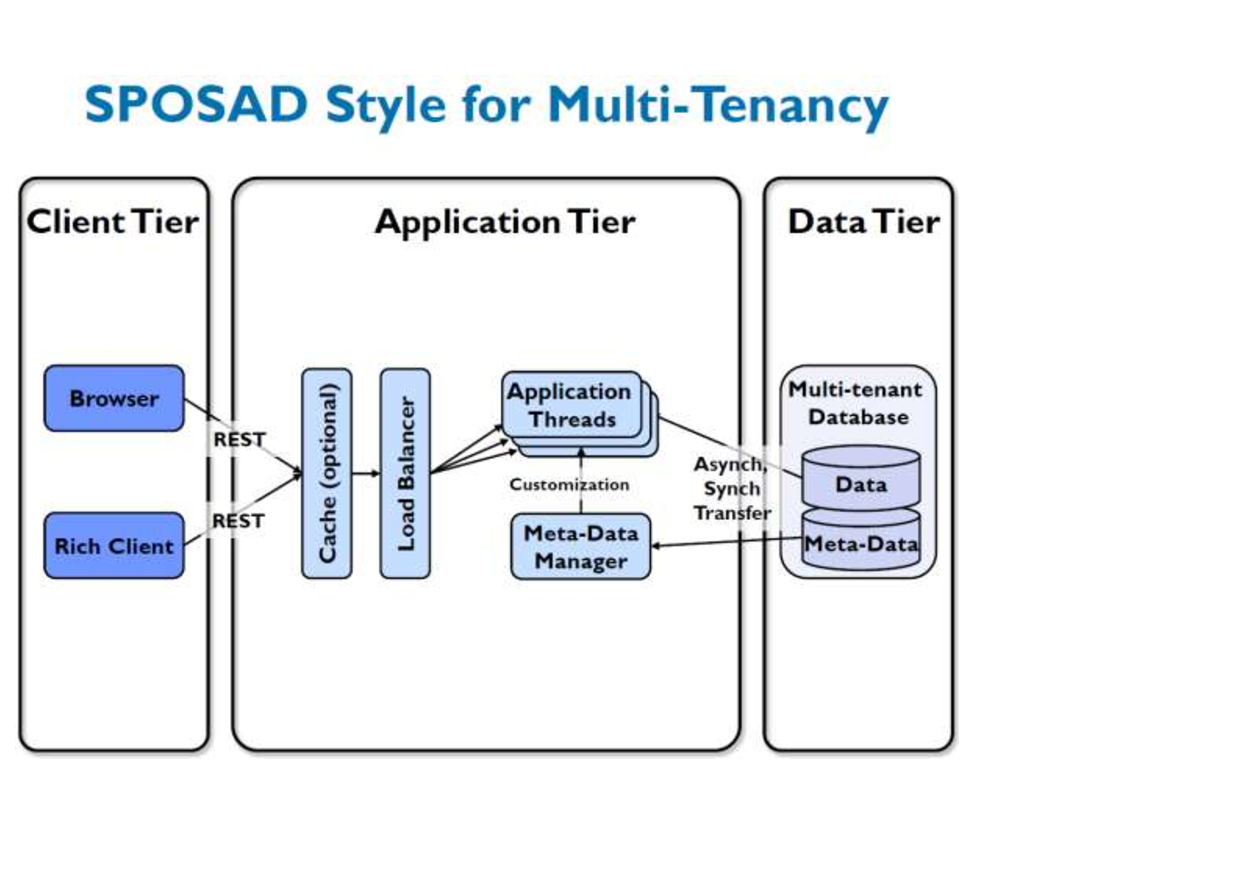
\includegraphics{patterns/Multi-tenantApplicationDiagram-01.pdf}
\caption{SPOSAD Style for Multi-Tenancy}
\label{fig:Multi-tenantApplicationDiagram-01}
\end{figure}

Figure \ref{fig:Multi-tenantApplicationDiagram-01} shows the inherent relation of the SPOSAD style to the n-tier architectural style, as it features a client, application, and database tier. Clients using web browsers or rich client applications interact with the application tier, which in turn accesses the database tier. The polymorphic application threads are the heart of the application tier. A load balancer directs user requests to them. The meta-data manager ensures that tenant-specific customizations are included in the application. The data tier differs from traditional n-tier architecture in the arrangement of the data, which is stored in a multi-tenant database that allows maximal resource sharing.

Requirements for a multi-tenant architecture are [Heiko Koziolek, 2010?]:
\begin{itemize}
	\item Resource Sharing: hardware and software resources, such
as hardware infrastructure, virtual machines, operating systems, databases, and code.
	\item Scalability: due to the inherent limits of scaling up (i.e., adding resources to a single node), the ability to seamlessly scale out (i.e., adding more nodes) is a typical architectural property of a multi-tenant system.
	\item Maintainability: shared code basis for several tenants. This feature helps to decrease the maintenance effort for the software,
because bugs only need to be fixed once and updates can be installed centrally. The multitenant design with a shared database also reduces costs for database administration and maintenance, which does not have to be executed for each tenant.
	\item Customizability: ability to incorporate tenant-specific customizations. Because of the shared application code base
and shared database it is not trivial to allow tenants to adapt the application's business logic and data to the requirements of their clients. A well-designed multi-tenant architecture is able to find a good trade-off between resource sharing and user customizability.
	\item Usability: the user interface shall be configurable through tenant-specific customizations. It allows different tenants to create their own branding for an application.
\end{itemize}

One of the implementation issues that comes from the aforementioned requirements is to have a database table column which holds the tenant ID.

\begin{figure}[h]
\centering
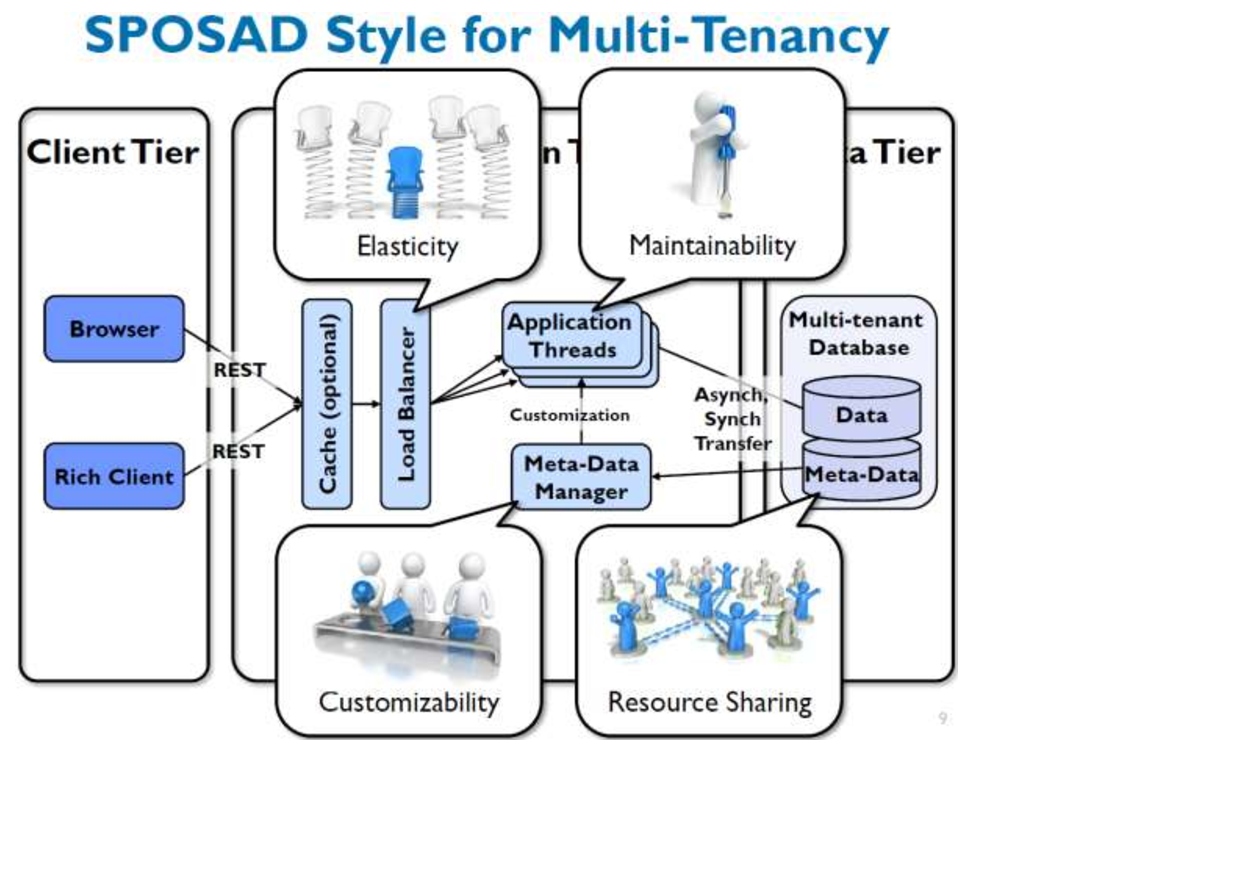
\includegraphics{patterns/Multi-tenantApplicationDiagram-02.pdf}
\caption{SPOSAD Style for Multi-Tenancy}
\label{fig:Multi-tenantApplicationDiagram-02}
\end{figure}

Force.com: With the force.com platform developers may build applications on top of the salesforce.com infrastructure. On a high abstraction level, the platform is built according to an n-tier architecture [WB09] comprising a presentation tier (using web browsers), an application tier, and a data tier.

Clients access the application tier of force.com according to the REST style. Each tenant is served by application instances originating from the same code base. Salesforce manages updates of this code base centrally. Tenants can customize the application user interface
(forms), business logic (workflows), and data (customized tables) by specifying metadata stored in the so-called Universal Data Dictionary (UDD). A runtime engine generates tenant-specific application code from this meta-data. Thus, the application is considered 'polymorphic', as it appears and behaves differently for the clients of each tenant.

Through the application tier, all tenants access the same logical database in the data tier. All tenant data is stored in a single table, which can be partitioned among multiple machines. Besides a tenant id column, the table contains 500 customizable columns (varchar
datatype) for storing arbitrary data (i.e., a universal table layout [AGJ+08]). Information about tenant-specific entities is stored in an additional 'objects' meta-data table, while information about tenant-specific fields is stored in an additional 'fields' meta-data table.
